\chapter{Deep noise suppression}
\label{ch:cfmse}
\note{XXXX}, the noisy observation can enter through the initial state, the conditioning input, or both. On VoiceBank--DEMAND, the noisy and clean speech have the same representation, so the noisy observation can serve as the starting point of a path towards clean speech. The experiments compare path shapes, including the effect of depth-dependent variance, and assess when a flow-trained model can be used for one-evaluation direct prediction. On CHiME-9 ECHI, the model receives four microphone signals and speaker enrolment and estimates a single target signal. A Gaussian source lets the flow evolve a mono state while receiving the multichannel observation through conditioning.

Related work applies flow matching to speech enhancement through several distinct design choices. FlowSE uses conditional flow matching to reduce the number of function evaluations required for enhancement \citep{leeFlowSEFlowMatchingbased2025}. \citet{korostikModifyingFlowMatching2025} investigate an informed source prior, a data-prediction objective, deterministic generation, and early stopping, including a deterministic one-step configuration for denoising. Their results also distinguish denoising from dereverberation, for which stochastic generation without the informed prior is preferable. These changes concern the source distribution, prediction objective, and generation procedure, rather than path variance alone.

FlowAVSE combines acoustic and visual conditioning with conditional flow matching for single-step audiovisual speech enhancement \citep{jungFlowAVSEEfficientAudioVisual2024}. Complementary work on generative speech foundation models pretrains a restoration model directly on complex-valued short-time Fourier transform coefficients and adapts it to tasks including denoising and target-speaker extraction \citep{kuGenerativeSpeechFoundation2025}.

\note{Remember to read the latest in flow amtching SE.}

\note{Maybe report +/- compared to the noisy instead of absolute value?}


\section{VoiceBank--DEMAND experiments}
\subsection{Metrics}
Speech quality is evaluated with intrusive and non-intrusive metrics. The intrusive speech-enhancement metrics are \ac{PESQ}~\citep{rixPerceptualEvaluationSpeech2001}, \ac{ESTOI}~\citep{jensen2016algorithm}, and \ac{SI-SDR}~\citep{leroux2018sdr}. SI-SDR is measured in dB. The evaluation also includes non-intrusive metrics that estimate quality from the enhanced speech alone: DNSMOS~\citep{reddy2021dnsmos},\footnote{https://github.com/microsoft/DNS-Challenge/tree/master/DNSMOS} a neural predictor trained on human ratings (\ac{MOS}), and WhiSQA, a non-intrusive \ac{MOS} predictor reported to correlate with human judgments \citep{closeHallucinationPerceptualMetricDriven2024,close2025whisqanonintrusivespeechquality}.\footnote{https://github.com/leto19/WhiSQA} Evaluation of a model takes all of these metrics into consideration, as simply optimising a single metric does not result in high quality SE \citep{deoliveira2024pesqetarian}. Higher scores indicate better quality for all metrics used here.


\subsection{Data}
The models in this section are trained and tested on the \ac{VB-DMD} dataset~\citep{valentini2016investigating}, a common benchmark for \ac{SE} containing clean speech recordings from 28 speakers with added background noise, e.g. caf\'e, traffic. Speakers p226 and p287 are used for validation. Non-intrusive evaluation of the clean speech yields 3.53 DNSMOS and 4.53 WhiSQA.

\note{URGENT not explained.}

\subsection{Models}
Here, path velocity denotes the derivative of the conditional path mean with respect to depth $u$. Static variance means variance that is independent of $u$. Data prediction (DP) and flow matching (FM) denote training objectives, whereas \ac{DDP} denotes an inference scheme.
Following \cite{jukic2024schr}, the original path-comparison models are trained until validation SI-SDR converges, after which the checkpoint with the best validation PESQ is selected. Unless otherwise stated, \ac{ODE} samplers are run for 50 steps, with batch size 8 and the same STFT settings as \cite{richterInvestigatingTrainingObjectives2025}.
In the original path comparison, the neural estimator $\rmF_\vtheta$ employs the NCSN++ architecture \citep{song2021sde} using the same parameterisation described in \cite{richter2023speech}. The original path comparison uses the time-domain auxiliary loss \citep{jukic2024schr}.

\subsection{Full-data comparison}
\note{Stay consistent with my original work and only report the P.808 DNSMOS not OVRL.}

\note{Why doesn't table cfmse-local have sbve? and why only historical sgmse? I don't see sgmse++ either.}

\note{Maybe consider using best, second best and worst colours like in part II? (obviously put noisy row in red)}

\begin{table}[htbp]
\centering
\small
\resizebox{\linewidth}{!}{%
\begin{tabular}{lrrrrrrrr}
\toprule
Model & Generation & NFE & PESQ & ESTOI & SI-SDR & OVRL & P.808 & WhiSQA \\
\midrule
Noisy & -- & 0 & 1.968 & 0.787 & 8.449 & 2.682 & 3.085 & 3.122 \\
Direct U-Net & Direct & 1 & 2.787 & 0.873 & 19.493 & 3.186 & 3.565 & 4.351 \\
Noisy-source ICFM & DDP & 1 & 2.949 & 0.878 & 19.937 & 3.187 & 3.590 & 4.498 \\
Noisy-source ICFM & ODE & 50 & 2.853 & 0.880 & 19.870 & 3.216 & 3.594 & 4.499 \\
Gaussian FM & DDP & 1 & 2.837 & 0.867 & 18.782 & 3.185 & 3.574 & 4.481 \\
Gaussian FM & ODE & 50 & 2.993 & 0.868 & 17.823 & 3.186 & 3.573 & 4.520 \\
Fixed-time ICFM & DDP & 1 & 2.850 & 0.873 & 19.330 & 3.186 & 3.584 & 4.433 \\
Annealed DDP & DDP & 1 & 2.903 & 0.877 & 19.510 & 3.200 & 3.581 & 4.464 \\
Fine-tuned DDP & DDP & 1 & 2.927 & 0.878 & 19.624 & 3.192 & 3.585 & 4.498 \\
SGMSE (historical) & -- & -- & 2.562 & 0.852 & 15.883 & -- & -- & -- \\
\bottomrule
\end{tabular}}
\caption{VB-DMD full-data baselines and flow models on 824 test utterances. Local rows use channel 0 and whole utterances. Both FM checkpoints use a waveform $L_1$ weight of 0.001. The historical SGMSE row comes from a separate evaluation. Dashes indicate unavailable or inapplicable entries. OVRL denotes DNSMOS overall.}
\label{tab:cfmse-local}
\end{table}

For the noisy-source ICFM checkpoint, switching from 50 ODE evaluations to one-evaluation DDP increases PESQ by 0.096 (95\% paired bootstrap interval 0.085 to 0.107). For the Gaussian FM checkpoint, the same switch decreases PESQ by 0.157 (interval for the signed difference $-0.175$ to $-0.138$). These intervals quantify variation across the 824 paired test utterances for the fitted checkpoints. The two checkpoints also differ in path and optimisation, so the reversal cannot be attributed to the source alone.

At one evaluation, noisy-source ICFM with DDP improves PESQ from 2.787 to 2.949 and SI-SDR from 19.493 to 19.937~dB relative to the direct U-Net in Table~\ref{tab:cfmse-local}.

\subsection{Original path comparison}
Table~\ref{tab:results} reports the original experiment on path and training objective. Its legacy DNSMOS output is labelled as recorded because the specific output could not be verified.

\begin{table}[htbp]
\centering
\resizebox{\linewidth}{!}{%
\begin{tabular}{cllll|ccccc}
        \toprule
               Path& Loss&Generation& k&$c$&  PESQ &  ESTOI &  SI-SDR&   DNSMOS&WhiSQA \\
    \midrule
     Noisy& -&-&-&-& 1.97& 0.79& 8.4&  3.05&3.11\\
             \midrule
    SB-VE& DP&ODE& 2.6&0.4& 2.92& 0.87& 19.3& 3.56 & 4.46\\
     SB-VE&  DP&ODE& 0.99& 0.375& 2.92 & 0.88 & 19.5& 3.56 &4.47 \\
             \midrule
    SB-SV& DP&ODE& 2.6&0.15& 2.98 & 0.88 & 19.4 & 3.58   & \textbf{4.51   }\\
    SB-SV& DP&ODE& 0.99&0.1& 2.86 & 0.88 & 19.5 & 3.58   & 4.47   \\
    ICFM& DP&ODE& -&0.1& 2.98 & 0.88 & 20.1 & 3.59  & 4.49\\
    ICFM& FM&ODE& -&0.1& 2.91 & 0.88 & 20.3 & \textbf{3.60} & 4.50 \\
    \midrule
             SB-VE   & DP&DDP& 2.6&0.4&  2.92&  0.87&  19.4&   3.55&4.45\\
             SB-SV& DP&DDP& 2.6&0.15& 2.98& 0.88& 19.9&  3.58&4.50\\
             SB-SV& DP&DDP& 0.99&0.1& 2.99& 0.88& 20.0&  3.57&4.50\\
             ICFM& DP&DDP& -&0.1&  \textbf{3.05}&  0.88&  20.2&   3.58&\textbf{4.51}\\
            ICFM& FM&DDP& -&0.1&  3.00&  0.88&  \textbf{20.4}&   3.59&\textbf{4.51}\\
            \bottomrule
        \end{tabular}
}
\caption{Mean speech quality metrics in the original \ac{VB-DMD} experiment for SB-SV and ICFM under the listed objectives and generation procedures, compared with the SB-VE \citep{jukic2024schr} baseline. $k=0.99$ induces straightness and $c$ scales variance.}
\label{tab:results}
\end{table}
The results are displayed in \tableref{tab:results}. The tested SB-SV and ICFM settings improve several metrics over the SB-VE baseline, but the table does not show improvement on every metric. Using SB-SV with $k=0.99$ lowers PESQ and WhiSQA relative to $k=2.6$. ICFM with depth-independent path velocity and variance improves several reported scores. For ODE inference, FM loss gives a slightly higher SI-SDR and DNSMOS than DP, while DP gives higher PESQ; for DDP, DP has the highest PESQ and FM has the highest SI-SDR. These results do not establish a single objective as superior on all metrics.
\begin{figure}[tb]
\centering
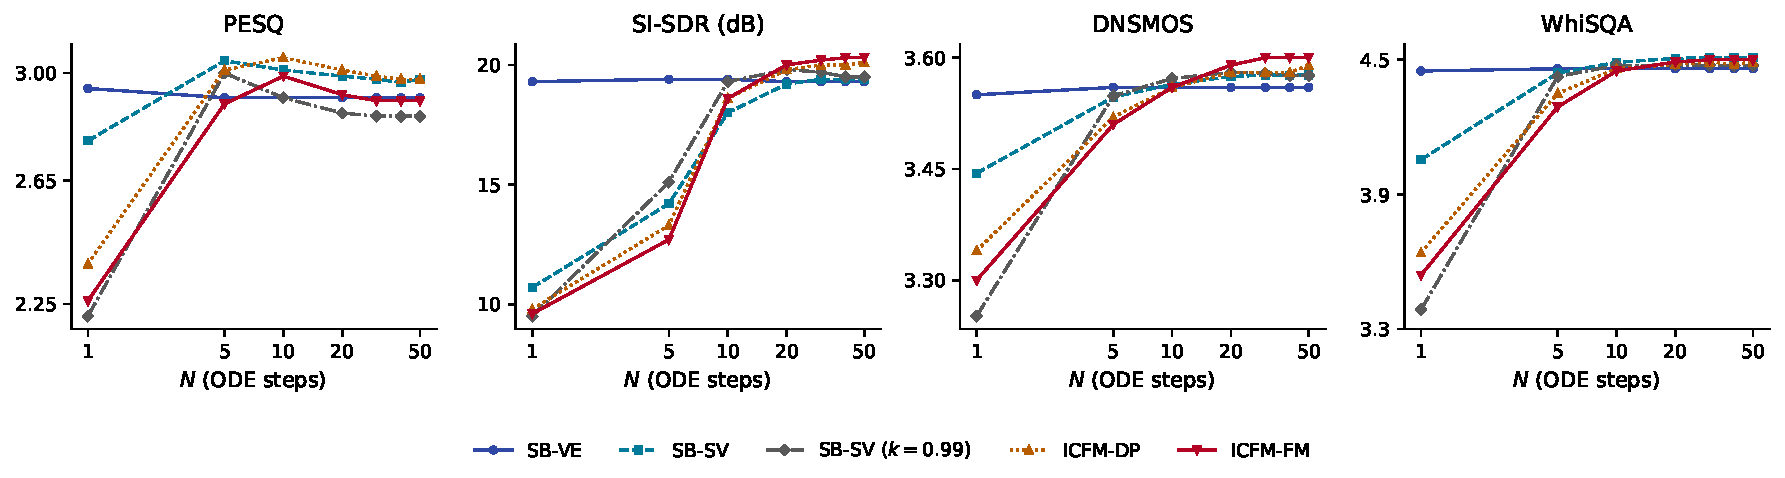
\includegraphics[width=\linewidth]{plots/se/ode_step_metrics.pdf}
\caption{Speech-enhancement quality against the number of ODE sampling steps $N$ on a logarithmic axis. Panels show PESQ, SI-SDR, DNSMOS, and WhiSQA, ordered from left to right and top to bottom. Unqualified SB-VE and SB-SV curves use $k=2.6$; the second SB-SV curve uses $k=0.99$. ICFM-DP and ICFM-FM denote the two training objectives. Higher scores indicate better quality.}
\label{fig:se-ode-steps}
\end{figure}
Figure~\ref{fig:se-ode-steps} compares the supplied ODE-step results. The $N=1$ points represent one-step ODE sampling; DDP results are reported separately in \tableref{tab:results}.

\subsection{ODE evaluation budget}
\begin{figure}[tb]
\centering
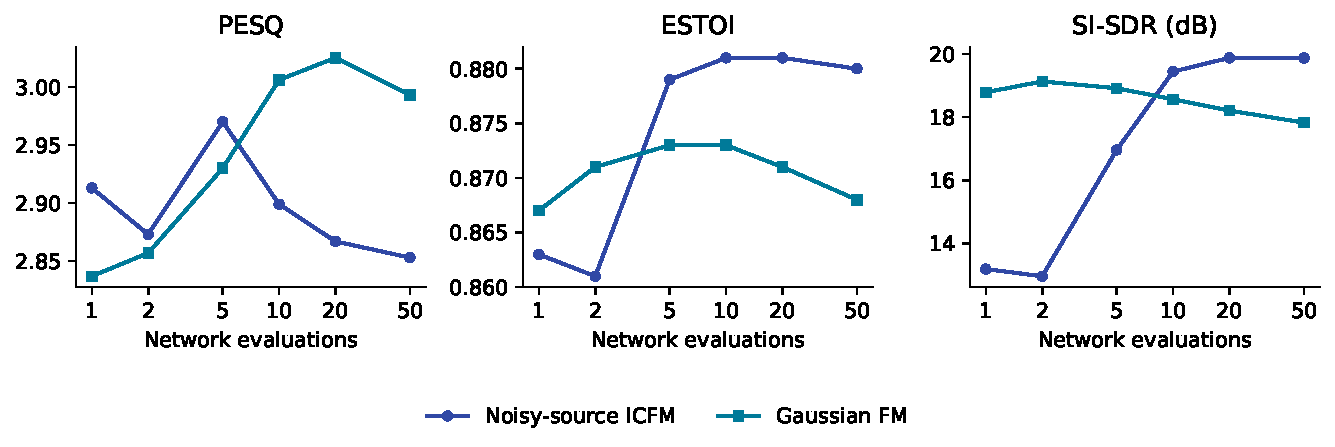
\includegraphics[width=\linewidth]{plots/se/vbdmd_atlas_nfe.pdf}
\caption{VB-DMD test results for the two flow-matching checkpoints in Table~\ref{tab:cfmse-local} across ODE evaluation budgets. Each point uses 824 utterances. The one-evaluation points use the ODE sampler. \note{Need dnsmos and whisqa too.}}
\label{fig:vbdmd-atlas-nfe}
\end{figure}
In Figure~\ref{fig:vbdmd-atlas-nfe}, noisy-source ICFM gains most of its SI-SDR by ten evaluations. Gaussian FM reaches its highest PESQ at 20 evaluations, while its SI-SDR peaks at two. These budgets were compared on the test set.

\subsection{Training speaker count}
Each training subset was used for 300 epochs. Smaller subsets therefore received fewer optimiser updates, so the sweep varies both the number of speakers and the optimisation budget.

\begin{table}[htbp]
\centering
\small
\begin{tabular}{lrrrrr}
\toprule
Model & 1 & 3 & 7 & 13 & 26 \\
\midrule
ICFM & 1.760 & 1.810 & 2.100 & 2.120 & 2.170 \\
SB-VE & 1.880 & 1.910 & 2.170 & 2.260 & 2.390 \\
SGMSE & 1.750 & 1.910 & 1.860 & 1.900 & 1.910 \\
SGMSE+ & 2.160 & 2.380 & 2.480 & 2.480 & 2.520 \\
\bottomrule
\end{tabular}
\caption{Best validation PESQ by number of training speakers.}
\label{tab:cfmse-data-3}
\end{table}
\begin{table}[htbp]
\centering
\small
\begin{tabular}{lrrrrr}
\toprule
Model & 1 & 3 & 7 & 13 & 26 \\
\midrule
ICFM & 12.187 & 11.852 & 16.091 & 16.761 & 18.011 \\
SB-VE & 10.676 & 15.326 & 16.417 & 16.337 & 17.457 \\
SGMSE & 12.977 & 13.723 & 12.859 & 12.633 & 13.715 \\
SGMSE+ & 13.572 & 15.008 & 14.845 & 14.292 & 14.977 \\
\bottomrule
\end{tabular}
\caption{Final validation SI-SDR (dB) by number of training speakers.}
\label{tab:cfmse-data-6}
\end{table}

Best validation PESQ is recorded to the precision of the checkpoint filenames. Final SI-SDR comes from the final epoch on 20 validation utterances. The two tables describe different checkpoint summaries. SGMSE+ retains higher PESQ across the subsets, while ICFM exceeds SGMSE+ in final SI-SDR at 7, 13, and 26 speakers. SB-VE has the highest final SI-SDR at seven speakers (16.417~dB).

\note{this table is stupid, we need real metrics not validation pesq.}

\subsection{Explicit observation conditioning}
\begin{table}[htbp]
\centering
\small
\begin{tabular}{lrrr}
\toprule
Model & PESQ & ESTOI & SI-SDR \\
\midrule
Direct U-Net & 2.377 & 0.771 & 16.946 \\
Fixed-time ICFM & 2.386 & 0.768 & 16.858 \\
ICFM, no explicit condition & 1.918 & 0.749 & 16.790 \\
SB-VE, no explicit condition & 2.187 & 0.736 & 15.350 \\
SGMSE, no explicit condition & 1.086 & 0.180 & -25.404 \\
\bottomrule
\end{tabular}
\caption{Conditioning ablations on 770 VB-DMD validation utterances. SGMSE uses 30 predictor--corrector steps. The other rows use one network evaluation.}
\label{tab:cfmse-conditioning}
\end{table}

At the noisy endpoint, DDP can evaluate $F_\theta(y,y,1)$ in the convention where the noisy endpoint is at depth 1, with the same observation supplied as both state and explicit condition. These inputs coincide at that endpoint, but have different roles during optimisation. At intermediate depths the state contains interpolated speech and perturbations, while the conditioning input still provides the original observation. Removing that input changes the information available during optimisation even when the observed endpoint remains the same. The ablated ICFM obtains 1.918 PESQ and 16.790~dB SI-SDR. The fixed-time ICFM obtains 2.386 PESQ and 16.858~dB SI-SDR under a different training protocol. The ablated SGMSE scores poorly across the three metrics. Estimating the effect of conditioning requires a conditioned counterpart for each ablated checkpoint, with the same training protocol and generation procedure.

\subsection{Out-of-distribution evaluation}
\begin{table}[htbp]
\centering
\small
\begin{tabular}{lrrrr}
\toprule
Model & Blind OVRL & Blind WhiSQA & Nonblind OVRL & Nonblind WhiSQA \\
\midrule
Noisy &  1.704 & 1.818 & 1.937 & 2.168 \\
Fine-tuned DDP &  2.673 & 2.303 & 3.038 & 3.306 \\
Noisy-source ICFM &  2.852 & 2.474 & 3.130 & 3.445 \\
Direct U-Net &  2.616 & 2.103 & 3.007 & 2.988 \\
Official SB-VE m5 &  2.820 & 2.256 & 3.147 & 3.216 \\
\bottomrule
\end{tabular}
\caption{URGENT transfer results for selected VB-DMD checkpoints, with 1,000 recordings per split. ICFM and SB-VE use 50 ODE evaluations. The direct U-Net and fine-tuned DDP use one evaluation.}
\label{tab:cfmse-urgent}
\end{table}

URGENT was evaluated on channel 0 at 16~kHz using four-second windows with 0.5-second overlap. Noisy-source ICFM at 50 ODE evaluations achieves higher WhiSQA than the one-evaluation direct U-Net on both splits.

\note{Why not include the original ICFM model. The choice of models in these tables seems completly random... SBVE and ICFM are available in the data efficiency experiment if the originals are archived.}

\section{CHiME-9 ECHI experiments}
A single-microphone transfer evaluation would measure how a mono enhancement model transfers to CHiME-9 recordings. The ECHI experiments instead use models optimised for extraction of the enrolled speaker from four microphone signals.

\subsection{Four-microphone conditioning and a mono state}
The ECHI models estimate a single complex speech STFT conditioned on four fixed microphone STFTs and target-speaker enrolment audio. A data-to-data path needs endpoints in a shared state space. A path starting from the multichannel observation therefore requires a channel selection, a projection to mono, or a state representation that accommodates both endpoints. With a Gaussian source, the evolving state can have the shape of the mono target throughout, while spatial and speaker information enter through the condition. The development experiment compares Gaussian-source paths and direct prediction.

For OT-FM, let $X$ denote the clean compressed spectrum and let $\epsilon$ be standard circular complex Gaussian noise with the same shape. With depth $u$ increasing from noise to speech, the path state is $(1-u)\epsilon+uX$ and the regression target is $X-\epsilon$. Euler generation starts from $\epsilon$.

The matched systems use a seven-level, width-64 NCSN++ backbone with a speaker encoder. The frontend uses a 510-sample Hann window and a 128-sample hop at 16~kHz. Evaluation uses four-second windows with two-second stride and normalised overlap-add. The development set contains 4,309 target-speaker segments and includes the subset used for checkpoint selection.
\begin{table}[htbp]
\centering
\small
\begin{tabular}{lrrrrrr}
\toprule
Model & NFE & PESQ-WB & STOI & SI-SDR & DNSMOS & WhiSQA \\
\midrule
GridNet & 1 & 1.075 & 0.384 & -35.625 & 1.087 & 1.454\\
Direct & 1 & 1.142 & 0.492 & -24.589 & 1.951 & 1.520\\
OT-FM & 1 & 1.122 & 0.531 & -23.767 & 1.825 & 1.546\\
Cosine & 1 & 1.091 & 0.483 & -23.889 & 1.849 & 1.529\\
VE & 1 & 1.075 & 0.325 & -37.883 & 1.871 & 1.579\\
ICFM & 1 & 1.138 & 0.512 & -23.304 & 1.787 & 1.566\\
SBVE adaptation & 1 & 1.117 & 0.364 & -45.718 & 1.090 & 1.452\\
\midrule
OT-FM & 16 & 1.215 & 0.587 & -27.953 & 2.542 & 1.911\\
Cosine & 16 & 1.131 & 0.501 & -27.906 & 2.325 & 1.729\\
VE & 16 & 1.078 & 0.255 & -41.289 & 1.780 & 1.323\\
ICFM & 16 & 1.123 & 0.499 & -26.422 & 2.081 & 1.717\\
SBVE adaptation & 16 & 1.091 & 0.492 & -32.719 & 1.440 & 1.609\\
\bottomrule
\end{tabular}
\caption{CHiME-9 ECHI development results at matched budgets of one and 16 network evaluations. Direct and GridNet are one-evaluation references. NFE counts evaluations per window. Means use the valid segments for each metric.}
\label{tab:cfmse-echi}
\end{table}

\note{Why not eval SBVE?}

\begin{figure}[tb]
\centering
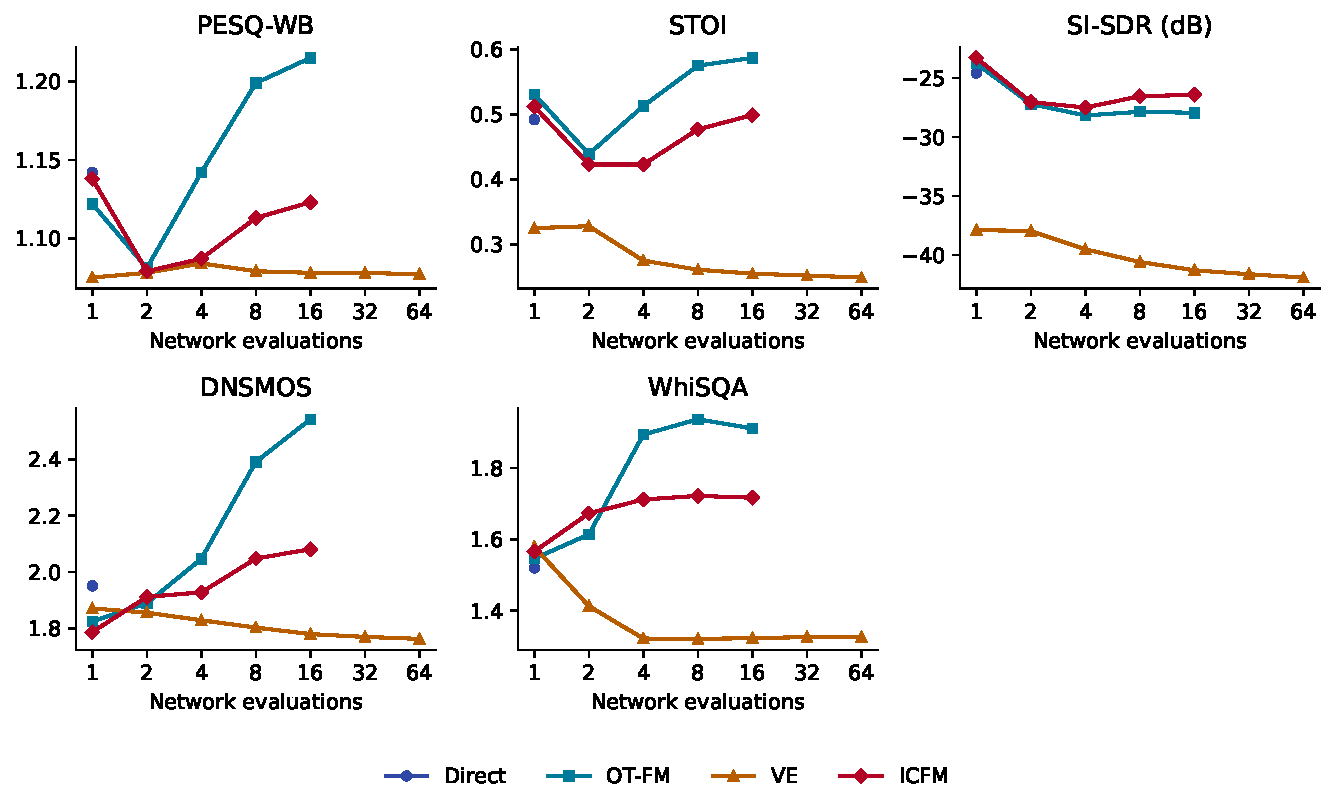
\includegraphics[width=\linewidth]{plots/se/echi_euler_nfe.pdf}
\caption{CHiME-9 ECHI development metrics by Euler evaluation budget for OT-FM, Gaussian-source VE, and normalised ICFM. The direct predictor is shown as a one-evaluation reference.}
\label{fig:echi-euler-nfe}
\end{figure}
Increasing the OT-FM budget from one to 16 evaluations raises STOI from 0.531 to 0.587 and wideband PESQ from 1.122 to 1.215, while SI-SDR falls from $-23.767$ to $-27.953$~dB. The eight-evaluation setting gives its highest WhiSQA (1.937), and one-evaluation ICFM gives the highest SI-SDR ($-23.304$ dB) among the reported systems. SI-SDR is negative across the reported systems under the official reference protocol without lag search. The OT-FM STOI gain over GridNet at 16 evaluations is 0.204 on 4,307 common valid segments, with a paired 95\% bootstrap interval of 0.197 to 0.210. The experiment uses one optimisation seed. Held-out evaluation remains unavailable because the local archive lacks the speaker assignments and enrolment audio required by the conditioned systems.

The ECHI development results demonstrate that a Gaussian source in the mono target space supports extraction conditioned on four microphones and speaker enrolment. A comparison with a data-to-data path under the same multichannel conditioning and evaluation protocol remains open.
